% !TeX spellcheck = en_GB
\documentclass[runningheads,a4paper]{llncs}
\usepackage[utf8]{inputenc}
\usepackage[T1]{fontenc}
\usepackage{csquotes}
\usepackage[english]{babel}
\usepackage[backend=bibtex,natbib,hyperref=true,maxnames=2,style=authoryear-comp]{biblatex}
%\usepackage[backend=biber,style=alphabetic-verb,citestyle=authoryear]{biblatex}
%\addbibresource{imagenet_trained_cnns_biased_towards_texture_seminarreport-blx.bib}
\addbibresource{Literaturverzeichnis.bib}

\usepackage{amsmath}
\usepackage{booktabs}
\usepackage{enumitem}
\usepackage{graphicx}
\usepackage{eurosym}
\usepackage[hidelinks]{hyperref}
\usepackage[capitalise]{cleveref}



\DeclareMathOperator*{\somefunc}{somefunc}
%


% USEFUL NOTES BEGIN ------------------------------------------------------------

%\begin{align} a^2 + b^2 = c^2, \end{align}

% Citation: \citep{Bailey}

%``quotes'' 

% \emph{italics}

%\begin{figure}[tbp]
%    \centering
%    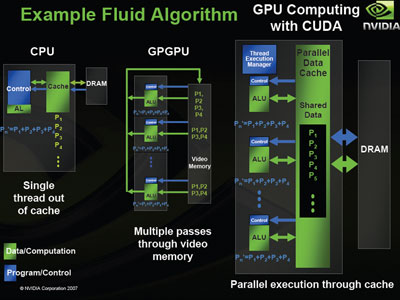
\includegraphics[width=.5\linewidth]{pic/cuda.jpg}
%    \caption{Something about CUDA architecture. Quite interesting.}
%    \label{fig:cuda}
%\end{figure}

%    \begin{table}
%        \centering
%        \begin{tabular}{@{}lrr@{}} 
%            \toprule
%            \multicolumn{2}{c}{Education}\\ \cmidrule{1-2}
%            Major & Duration & Income (\euro)\\ 
%            \midrule 
%            CompSci & 2 & 12,75 \\ \addlinespace
%            MST & 6 & 8,20 \\ \addlinespace
%            VWL & 14 & 10,00\\ 
%            \bottomrule
%        \end{tabular}
%        \caption[Table Example]{A basic example from the booktabs package.}
%        \label{tab::ex}
%    \end{table}

%\begin{abstract} \end{abstract} \section{Introduction} \section{Related Work} \section{Methods} \section{Results} \section{Conclusion}

% USEFUL NOTES END ------------------------------------------------------------

%TODO: QUESTIONS:
% - 

\begin{document}
%
\frontmatter          % for the preliminaries
%
\pagestyle{headings}  % switches on printing of running heads
%
\mainmatter              % start of the contributions
%
\title{Article review: IMAGENET-TRAINED CNNS ARE BIASED TOWARDS TEXTURE; INCREASING SHAPE BIAS IMPROVES ACCURACY AND ROBUSTNESS}
\subtitle{Seminar: Vision Systems MA-INF 4208 \\by prof. Sven Behnke and Hafez Farazi}
%
\titlerunning{Seminar: Vision Systems}  % abbreviated title (for running head)
%
\author{Beaumont, Fabrice}
%
\authorrunning{Beaumont, Fabrice}   % abbreviated author list (for running head)
\institute{Universit\"at Bonn\\
\email{s6fabeau@uni-bonn.de},
2747609
}

\maketitle              % typeset the title of the contribution

\begin{abstract}
	Convolutional Neural Networks (CNNs) are used for many Computer Vision tasks and yet not all factors of their success are fully understood. In this report I will summarize the results of the paper ``IMAGENET-TRAINED CNNS ARE BIASED TOWARDS TEXTURE; INCREASING SHAPE BIAS IMPROVES ACCURACY AND ROBUSTNESS'' \citep{geirhos2018imagenet} which was published as a conference paper at ICLR in 2019. The results that are presented in this paper indicate, that depending on the database used for training, CNNs can bias their classifications towards recognized shape or texture. The authors of this paper also find, that CNNs which are biased towards shape perform better, due to a better transfer learning and a higher tolerance of noise. I will conclude the summary with some criticism towards the argumentation and highlight some questions, which were left uncommented by the authors. At last I will offer some suggestions for future work, since this is missing in the summarized paper entirely.
\end{abstract}

\section{Introduction}

In this report I will summarize the paper ``IMAGENET-TRAINED CNNS ARE BIASED TOWARDS TEXTURE; INCREASING SHAPE BIAS IMPROVES ACCURACY AND ROBUSTNESS'' by Robert Geirhos, Patricia Rubisch, Claudio Michaelis, Matthias Bethge, Felix A. Wichmann and Wieland Brendel from 2018 \citep{geirhos2018imagenet}. \\
There are three main results of this paper. 
First, the authors conclude from a set of experiments that convolutional neural nets (CNNs) use textures for object classification on the ImageNet (IN) database. Secondly, they show that this texture-bias can be replaced by a shape-bias by using an adapted database. Finally, the authors present experiments, which indicate that CNNs with a shape-bias are more robust to unseen distortions and noise.\\

After the summary of this paper I will offer some criticism on it and give some inspiration for future work.


\subsection{The object classification task}
%(till 1. page)
Object classification and semantic segmentation are common tasks in Computer Vision.  CNNs have been regarded as the closest model of the human vision (\cite{kubilius2016}, \cite{ritter2017cognitive}, \cite{cadieu2014deep} and \cite{yamins2014performance}) and are taken to be suited for object classification and other related tasks (\cite{krizhevsky2012imagenet}, \cite{long2015fully}).

The fundamental question, which the experiments of the authors should answer, was on which visual cues a CNN bases its classification. To guide the experiments, they identify two different hypothesis as possible answers to this fundamental question. The hypotheses state, that a CNN bases its classification either on the shape or the texture which is found in the presented image. They refer to these opposing answers as the shape and the texture hypothesis and base them on different findings in a couple of publications.

The authors stress, that the shape hypothesis is considered as ``one widely accepted intuition'' \citep{geirhos2018imagenet}. Furthermore, it would justify the usage of CNNs as a model of the human ventral system (\cite{cadieu2014deep}, \cite{yamins2014performance}). On the other hand, the authors refer to much more literature, which indicates that the texture hypothesis might be more accurate.

Since the authors present a variety of different related work in context of these two hypotheses throughout their paper, I will give a compact overview about it in the next section.

\section{Related work}

\subsection{Shape hypothesis}
The shape hypothesis states, that CNNs base their image classification on the shape of an object, found in a presented image. Publications, which indicate that this hypothesis is true and which were used by the authors, are the following:\\
Visualizing the functionality of neural activities in CNNs indicates, that the networks learn to recognize object parts, which are often interpreted by researchers as shapes \citep{zeiler2014visualizing}. One such proposed method of visualization are Deconvolutional Networks. From another perspective, it has been proposed by \citet{ritter2017cognitive} and \citet{geirhos2018generalisation} that CNNs tend to use shape rather than color in order to categorize objects.

Furthermore, according to \citet{ritter2017cognitive}, \citet{cadieu2014deep}, \citet{yamins2014performance} and \citet{landau1988importance} CNNs are the most predictive models for the human ventral stream object recognition, which is biased towards object shape.

\subsection{Texture hypothesis}
The texture hypothesis states, that CNNs base their image classification on the texture, found in a presented image.  Publications, which were referred to by the authors and indicate that this hypothesis is true are the following:

\citet{hosseini2018assessing} argued, that CNNs perform significantly worse on images with reversed brightness (negative images) - which preserve all shapes from the original image. Thus they conclude that shape can not be the only deciding factor.

\citet{gatys2015texture}, \citet{gatys2017controlling}, \citet{brendel2019approximating}, \citet{ballester2016performance}, \citet{funke2017synthesising}, \citet{ballester2016performance} and  \citet{eckstein2017beyond} all observed, that CNNs continue to perform well, if the shape of the presented objects was distorted or missing. But they perform badly, if the texture is missing.

At last, \citet{wallis2017parametric}, \citet{laskar2018correspondence} and \citet{long2018role} argued, that the correlation between CNNs and the human ventral stream could be based around their ability to recognize texture and not shape.

With these publications in mind, Geirhos and his team aimed towards specifying the prominent cues on which classifications done by a CNN are based on. In the next section their methods to achieve this goal are summarized.

\section{Methods}
The authors present three major results. As indicated by their presentation in the paper, these results and the methods used to support them, follow a natural train of though. First, to investigate whether CNNs are biased towards shape or texture, the authors use the classifications of 97 humans (completing 48,560 psychophysical trials) as a comparison against the performance of four CNNs on the IN database. This comparison is reasonable, since it is supported by some publications that humans base their object recognition on shape, rather than texture (\cite{ritter2017cognitive}, \cite{landau1988importance}).

The used CNNs were AlexNet \citep{krizhevsky2012imagenet}, GoogLeNet \citep{szegedy2015going}, VGG-16 \citep{simonyan2014very} and ResNet-50 \citep{he2016deep}.

For these experiments, images in the six categories original, greyscale, silhouette, object shape, texture  and texture-cue conflict were presented to both the humans and the CNN. Images of the class original, were untempered images from the IN database. They show objects in natural color in front of a white background.
Images of the class greyscale, silhouette and object shape, were converted images from the original class. For this convertation the authors used \texttt{skimage.color.rgb2gray}, a series of command line convertations with commands like \texttt{convert} and \texttt{potrace}, manual adjustment to pixels of the images and the Canny edge extractor implemented in MATLAB.
For each of these classes 160 images were used. Images of the class texture were original images in natural color from the IN database, too. But they typically displayed patches of an animal or many repetitions of the same man-made objects. 48 of such pictures were used. Finally, images of the class texture-cue conflict were generated using the method called style-transfer (implemented by \citet{huang2017arbitrary} and originally proposed by \citet{gatys2016image}).
This method is used to merge the content of one picture - in this case an image from the class original - with the style of another picture - in this case an image from the class texture. The process strips the content picture of its texture and replaces it with the texture of the style picture. This way, the results contain shapes displaying one object and a texture that belongs to another object. 1280 of these images were used.

All images displayed an equal amount of shapes from 16 different categories, which belong to the so called 16-class-ImageNet categories \citep{geirhos2018generalisation}. These 16 categories are: \textit{airplane}, \textit{bear}, \textit{bicycle}, \textit{bird}, \textit{boat}, \textit{bottle}, \textit{car}, \textit{cat}, \textit{chair}, \textit{clock}, \textit{dog}, \textit{elephant}, \textit{keyboard}, \textit{knife}, \textit{oven} and \textit{truck}. Note that, for the images of the texture-cue conflict class, only the underlying shape image has to correspond to one of these categories.

\subsection{Experimental setup} 
The experimental setup for the four CNNs consisted of their training on the IN database. They then were used to classify the images of the described categories. 
Since these four CNNs are capable of recognizing 1,000 different classes (e.g. tiger cat and Egyptian cat), their answers were mapped onto the 16 simpler answers (e.g. cat).

For the evaluation of the human participants, each trial lasted 2200 ms and contained the display of a fixation square (300 ms), a stimulus image (200 ms), a full-contrast pink noise mask (200 ms) and a screen where the participants had to select one of the 16-class-ImageNet categories as their response to the stimulus image (1500 ms). Each participant was shown pictures of exactly one class only. The participants classifying images with an objective ground true (not the texture-cue conflict images) were motivated by an increase in payment, proportional to an accuracy above 50\%. The authors claim, that by following the paradigm of \citet{geirhos2018generalisation} they had achieved maximal comparability between the human participants and the CNNs.

\subsection{Result 1 - Supporting the texture hypothesis}%TODO: CONTINURE
The results indicate, that both the pre-trained CNNs and the human participants perform well in the classification, if at least the objects texture is present (classes original, greyscale and texture). If the texture is missing entirely (classes silhouette and edges) all performances are lower, but the human participants still had an accuracy above 75\% where as the algorithms had accuracies below 54\%. See figure 2 of \citet{geirhos2018imagenet} for reference.

When both a shape and a texture cue were present (texture-shape cue conflict class), the human participants showed a clear preference for the identification of the object whose shape was present. On the other hand, the decisions of the algorithms varied much more between recognizing the shape or the texture. The overall tendency however was towards the present texture. See figure 4 of \citet{geirhos2018imagenet} for reference.

The authors concluded, that CNNs in general are biased towards texture, whereas humans are biased towards shape. They argued, that this bias is not present by design of the network, but rather induced by the database used for training. Since one application for the CNNs is to model the human vision, the authors tried to shift the texture-bias towards a shape-bias, like it can be observed for humans.

%(till 4. page)
\subsection{Stylized ImageNet (SIN) database}
In order to shift the bias of the CNNs, the authors changed the database used for the training. The underlying strategy was to remove the information stored in the texture of the images and to only keep the information stored in the shape of the images intact. This way the texture information looses importance and the CNNs would have to rely on the shapes.

The authors used the same method like for the images in the texture-shape cue conflict class, but this time the source for the style images were the 79,434 paintings images in Kaggle's ``Painter by Number'' data set (\url{https://www.kaggle.com/c/painter-by-numbers/}, which the authors accessed on March 1, 2018). Using this approach, every image of the IN database was mapped exactly once onto a newly generated style-transfer version. This newly formed database is called Stylized ImageNet (SIN) and it is as large as the IN database.

\subsection{Result 2 - Switching to a shape-bias}

The experiments with the SIN database indicate, that the classification performed by the ResNet-50 which was trained on SIN has shifted towards the shape recognition (from 22\% to 81\%) when it comes to the texture-shape cue conflict class. They also hint at similar results for the Alexnet and VGG-16. See figure 5 of \citet{geirhos2018imagenet} for reference.

In the paper the authors argue, that a lower top-5 accuracy of the ResNet-50 trained and evaluated on the SIN database (79,0\%) than on the IN database (92.0\%) indicates, that the classification using only shape cues is more difficult (table 1 on \citet{geirhos2018imagenet}). Furthermore, since the evaluation on the other database lead to a significant performance drop if the CNN was trained on the IN database (16.4\%) but an increase if it was trained on the SIN database (82.6\%), the authors argue, that relying on shape is more effective and generalizes better than relying on texture.\\

When evaluating the performance of the CNN which was trained on the SIN database, again images constructed by a style-transfer were used. This time the originally proposed method \citep{gatys2016image} were used. It consists of an iterative approach and thus would take to much time to be applied to the whole IN database in order to create the SIN database. But using these two implementations allowed for more independent evaluation of the effectiveness of the training on the SIN database.

At last the authors used BagNets \citep{brendel2019approximating}, which are CNNs with a restricted receptive field and thus with a handicap when it comes to recognizing global shapes. The performance of these BagNets was significantly reduced when trained and evaluated on the SIN database. 

All these results were interpreted by the authors as the effectiveness of the SIN database. Meaning a good accuracy of classifying images on it demands a shape-bias and can be induced when it is used for training. Finally the authors tried to determine, if the training with the changed database improves the performance of the CNNs.

\subsection{Result 3 - Superiority of the shape-bias}

To create a most performant CNN, the authors used the ResNet-50 architecture, pre-trained and fine-tuned on the IN database and trained again on their SIN database. This way, they were able to improve the top-1 accuracy on the IN database from 76.13\% (without the training on the SIN database) to 76.72\%. The analogue top-5 accuracy was improved from 92.86\% to 93.28\%. Most impressive are however the reported results when the authors used a Faster R-CNN \citep{ren2015faster} implementation of the ResNet-50 and demonstrate the transfer learning capabilities of their CNN trained on the SIN database as described above. This way they increased the mean average precision or an intersection over union of 50\% from 70.7\% to 75.1\% on the Pascal VOC database and from 52.3\% to 55.2\% on the MS COCO database. See table 2 of \citet{geirhos2018imagenet} for reference.


At last the authors present, that while only training on the SIN database may lead to a slightly less accurate classification on untempered images, it is beneficial when some unseen noise is applied to the input images. This applied noise was uniform noise, a phase noise, a contrast filer, a high-pass filter and some Eidolon distortions. Only applying a low-pass filter is disadvantageous for the CNN which was trained on the SIN database. The authors argue that this could correspond to the 
induced shape-bias, since the low-pass filter blurs sharp edges and thus hides object shapes while keeping a lot of texture information intact. See figure 6 of \citet{geirhos2018imagenet} for reference.

\section{Conclusion}
The summarized paper by \citet{geirhos2018imagenet} presents experimental results which indicate that CNNs tend to use texture over shape for classification tasks, if the training database allows it. Using a modified database can increase the tendency of a CNN to classify images using the displayed shapes. If this is the case, the performance is increased and transfers better to unseen data including noise.

The authors demonstrate these findings for one kind of database adaptation using the ImageNet database, a style-transfer method and Kaggle's ``Painter by Number'' data set. They also focus on presenting experiments with implementations of ResNet-50.

%(till 6. page)
\section{Critic}
The overall structure of the paper is very clear and simple to follow. The train of thought leads the reader in a logical comprehensive way from one result to the next. All presented images, figures and tables support the understanding and underline the presented information.
On top of that, the appendix hints at more detailed findings and completes the main paper seamlessly.

Nevertheless there are some weak points of the paper. Most obvious is the missing section about future work and an outlook on how to use and further investigate the presented results.

Secondly, some assumptions regarding the first major result can be challenged. For example the authors interpret the lower top-5 accuracy of the ResNet50 trained and evaluated on the SIN database as an indication that classification by shape is more difficult for the algorithm. In this argumentation they seem to not consider, that based on their construction of the SIN database, some images may loose information about the displayed object shape during the style-transfer. Thus the algorithm has less reliable input to train and evaluate on. This leads to the following other weak point of the paper. The authors themselves do acknowledge that the style-transfer can lead to images without reliable information about the object shape, but they do not implement or suggest any methods to counter this problem. Since the underlying idea of the SIN database is to have reliable shape information, counter measures seem to be essential. One example would be to use high-pass filters or otherwise increase the clarity of edges and shapes. This could be done both before the style-transfer and later added to the image or afterwards. The methods to derive the object silhouette or the edge shapes could be applied too.
Next, the authors only experiment with one kind of style-transfer by relying on one database of pictures for the artificial textures only. It seems to be a natural question to ask how other kinds of style-transfer are able to change biases in CNNs.
Related to this question is, how other parameters such as changes to the architecture of the CNN or usage of loss functions can influence any present bias.

On a less general base, the authors do not comment what happened during the so called ``fine tuning''-step for the Shape-ResNet. It has a rather noticable positive effect on its performance. For the results with respect to the MS COCO this improvement is just slightly less, than the actual additional usage of the SIN itself.
On top of that, the reasons for the decision to focus on ResNet-50 are not very clear. While similar results with other CNNs are hinted at, the authors formulate the last two results as general statements, but only support the claims with results about this single CNN.

Experiments with adversarial input lead to a better understanding on how CNNs work \citep{zeiler2014visualizing}. Nevertheless the authors fail to report about any results of their trained CNN with this regard. However Geirhos himself stated for example in a dialogue with the British technology news cite ``The Register'', that their CNNs were still susceptible to such adversarial input (\url{https://www.theregister.com/2019/02/13/ai_image_texture/}, which the authors accessed on October 1, 2020).

Similarly, the authors hinted at related work of \citet{zeiler2014visualizing}, which support the shape hypothesis. For example with the argumentation that in CNNs a hierarchy of detected shapes is learned. The authors fail to comment on these interpretations which they claim to have indirectly outdated with their results.

The authors also state that all the images from the class original and texture were correctly classified by all four pre-trained CNNs. Thus it is misleading, that the perfect accuracy of the CNNs regarding the recognition task for not only the greyscale, silhouette, object shape and texture-cure conflict images, but also the original and texture images are presented. By construction the latter are recognized perfectly and thus this result gives no indication about the actual performance of the CNNs.

Lastly, some formulations in the paper are more general, than the actual presented results indicate. For example when the authors claim to have achieved the ``maximal'' comparability between the results of the humans and the four CNNs \citep{geirhos2018imagenet}. Since the humans can learn during their trial and the machines can not, there still should be at least some theoretical possibility to improve the comparability. An other example is the overall implication of the authors that their results on a few CNNs and a few databases would seamlessly generalize towards biases in all CNN. Although these formulations are probably not misunderstood by the intended audience, they could have been avoided.

\section{Future work}

From this paper one can derive many questions for future investigations with respect to the learning performed by CNNs. The authors only experimented with one kind of stylization by using one style-transfer method \citep{huang2017arbitrary} and one specific data base for the style images which consisted of paintings (Kaggle's ``Painter by Numbers''). \citet{hosseini2018assessing} experimented with the performance of CNNs on images that where modified in a different way. They used inverted images which loose some information about the original color but preserve all information about edges and thus shape. One could expand these experiments in order to investigate what kind of databases are most suited for what kind of recognition tasks. Also, it would be interesting to what extent the underlying decision process of CNNs can be determined by augmenting the training database.

In contrast to this, it remains unclear, if similar biases of CNNs can be induced by changing their architecture or introducing loss functions to the network. Afterwards one could try to combine several of these approaches to further guide the decision parameters of CNNs.

On the other hand, it could be disadvantageous to have CNNs that are strongly biased towards single cues like only object shape. Depending on the complexity of the target database it could be promising to add a decision layer for the CNNs, which applies classification mechanisms with different biases, depending on the already found information. The texture of some object are arguably more important than its shape. One very basic natural occurring example is the distinction between different panthers such as the black panther, a leopard or a jaguar.

As mentioned, the authors of the presented paper use the object classification task for their evaluation. The application and evaluation of their method to other related tasks in the field of Computer Vision could be investigated too. For example the task of semantic segmentation could be further specified, if different biases of the used CNNs lead to different but arguable useful segmentations.

At last, later published work like \citet{xie2020self} and \citet{xie2020adversarial} refer to the findings of \citet{geirhos2018imagenet} and claim to have improved the accuracy even further. This generally allows for more comparing studies, and for a further improved understanding of CNNs.

%Why was there no comment on Between-Class learning (Mix-up technique)? (e.g. Tokozume et al., 2018 and after the publication:  Bhattacharjee et al. 2020)Is it possible that different biases lead to categorically different object detections?\\


\printbibliography
\end{document}
